\documentclass[11pt,aspectratio=169]{beamer}

\usepackage[utf8]{inputenc}
\usepackage[T1]{fontenc}
\usepackage[spanish,es-tabla,es-nodecimaldot]{babel}
\usepackage{amsmath,amssymb}
\usepackage{newpxtext,newpxmath}
\usepackage{graphicx}
\usepackage{xcolor}
\usepackage{booktabs}
\usepackage{colortbl}
\usepackage{tikz}
\usetikzlibrary{arrows.meta,fit,backgrounds,calc,shapes.geometric,decorations.pathreplacing,positioning}
\usepackage[most]{tcolorbox}
\usepackage{multicol}

\graphicspath{{figures/}{informe/figures/}{./}{informe/}{../figures/}}

% ---------------------------------------------------------------------
% Paleta institucional UGR
% ---------------------------------------------------------------------
\definecolor{ugrAzul}{HTML}{0B3D91}
\definecolor{ugrCeleste}{HTML}{3FA9F5}
\definecolor{ugrRojo}{HTML}{E5323B}
\definecolor{ugrNaranja}{HTML}{E07B00}
\definecolor{ugrVerde}{HTML}{2E8B57}
\definecolor{ugrGris}{HTML}{6B7280}
\definecolor{filaResaltada}{HTML}{EAF2FB}
\definecolor{ugrFondoClaro}{HTML}{F5F9FD}

% ---------------------------------------------------------------------
% Estilos TikZ
% ---------------------------------------------------------------------
\tikzset{
    base/.style={rectangle, rounded corners=3pt, align=center, inner sep=4pt, line width=0.7pt},
    nodoES/.style={base, draw=ugrAzul, fill=ugrAzul!9, text width=3.3cm},
    nodoEN/.style={base, draw=ugrNaranja, fill=ugrNaranja!9, text width=3.3cm},
    proceso/.style={base, draw=ugrAzul, fill=white, text width=#1},
    resultado/.style={base, draw=ugrVerde, fill=ugrVerde!9, text width=#1},
    flecha/.style={-{Stealth[length=2.4mm, width=1.8mm]}, line width=0.8pt, color=ugrGris},
}

% ---------------------------------------------------------------------
% Configuración beamer
% ---------------------------------------------------------------------
\usetheme{default}
\setbeamersize{text margin left=0.6cm,text margin right=0.6cm}
\usefonttheme{serif}
\setbeamertemplate{navigation symbols}{}

\setbeamercolor{structure}{fg=ugrAzul}
\setbeamercolor{title}{fg=ugrAzul}
\setbeamercolor{frametitle}{fg=ugrAzul}
\setbeamercolor{section in toc}{fg=ugrAzul}
\setbeamercolor{normal text}{fg=black}
\setbeamercolor{block title}{fg=white,bg=ugrAzul}
\setbeamercolor{block body}{bg=ugrFondoClaro}

\setbeamertemplate{footline}
{
  \leavevmode\hspace*{0.6cm}\raisebox{-0.12cm}{
\includegraphics[height=0.45cm]{logo_ugr.png}}\hspace*{0.3cm}\footnotesize\textcolor{ugrGris}{\ifnum\value{section}>0 CRISP-DM $\cdot$ Fase \insertsectionnumber: \fi\insertsectionhead}\hfill\footnotesize\textcolor{ugrAzul}{\insertframenumber/\inserttotalframenumber}\hspace*{0.6cm}\vskip0.2cm
}
\setbeamerfont{caption}{size=\scriptsize}
\setbeamertemplate{section in toc}{\textcolor{ugrCeleste}{\bfseries\inserttocsectionnumber}\hspace{0.6em}\inserttocsection}

\setbeamertemplate{frametitle}
{
  \vskip0.1cm
  \begin{beamercolorbox}[wd=\textwidth,sep=0.2cm,vmode]{frametitle}
    \Large\bfseries\insertframetitle
  \end{beamercolorbox}
  \vskip-0.2cm
  \textcolor{ugrCeleste!40}{\rule{\textwidth}{2pt}}
  \vskip0.2cm
}

\newcommand{\ugrsubtitle}[1]{%
  \vskip-0.25cm
  \small\textcolor{ugrGris}{\emph{#1}}\par
  \vskip0.15cm
}

\setbeamertemplate{itemize/enumerate body begin}{\setlength{\itemsep}{0.1em}\setlength{\parskip}{0pt}}
\setbeamerfont{itemize/enumerate body}{size=\small}
\setbeamerfont{itemize/enumerate subbody}{size=\footnotesize}
\setbeamertemplate{itemize item}{\textcolor{ugrAzul}{\textbullet}}
\setbeamertemplate{itemize subitem}{\textcolor{ugrCeleste}{\textendash}}

\newcommand{\ugrblock}[2]{
  \begin{tcolorbox}[
    enhanced, colback=ugrFondoClaro, colframe=ugrAzul, boxrule=0.8pt, arc=3pt,
    title={\textbf{#1}}, fonttitle=\small\bfseries, coltitle=white, colbacktitle=ugrAzul,
    left=6pt, right=6pt, top=2pt, bottom=2pt, before skip=0.3em, after skip=0.2em
  ]
    #2
  \end{tcolorbox}
}

\newcommand{\ugrblockok}[2]{
  \begin{tcolorbox}[
    enhanced, colback=ugrVerde!8, colframe=ugrVerde, boxrule=0.8pt, arc=3pt,
    title={\textbf{#1}}, fonttitle=\small\bfseries, coltitle=white, colbacktitle=ugrVerde,
    left=6pt, right=6pt, top=2pt, bottom=2pt, before skip=0.3em, after skip=0.2em
  ]
    #2
  \end{tcolorbox}
}

\newcommand{\Hs}[1]{$H_{s\boldsymbol{#1}}$}

\newcommand{\tikzdiagram}[1]{
  \begin{center}
    \resizebox{0.95\textwidth}{!}{#1}
  \end{center}
}

\begin{document}

% =====================================================================
% PORTADA
% =====================================================================
\begin{frame}[plain]
  \begin{tikzpicture}[remember picture,overlay]
    \fill[ugrAzul] (current page.north west) rectangle ([yshift=-1.2cm]current page.north east);
    \node[anchor=west,text=white,font=\scriptsize\bfseries] at ([xshift=1.5cm,yshift=-0.6cm]current page.north west) {UNIVERSIDAD DEL GRAN ROSARIO};
    \node[anchor=east,text=ugrCeleste!40,font=\scriptsize] at ([xshift=-1.5cm,yshift=-0.6cm]current page.north east) {Licenciatura en Ciencia de Datos};

    \node[anchor=north east] at ([xshift=-1.2cm,yshift=-1.5cm]current page.north east) {
\includegraphics[width=3cm]{logo_ugr.png}};
    \fill[ugrCeleste] ([xshift=1.5cm,yshift=-2.7cm]current page.north west) rectangle ([xshift=1.56cm,yshift=-5.3cm]current page.north west);
    \node[anchor=north west,text width=0.66\paperwidth,text=ugrAzul,font=\fontsize{17}{21}\selectfont\bfseries,align=left] at ([xshift=2.0cm,yshift=-2.6cm]current page.north west) {Detección temprana de indicios de\\ depresión en español mediante PLN};
    \node[anchor=north west,text width=0.8\paperwidth,text=ugrGris,font=\footnotesize\itshape,align=left] at ([xshift=2.0cm,yshift=-4.4cm]current page.north west) {Evaluación empírica de modelos contextuales y líneas base clásicas};

    \draw[ugrGris!40,line width=0.4pt] ([xshift=1.5cm,yshift=2.9cm]current page.south west) -- ([xshift=-1.5cm,yshift=2.9cm]current page.south east);
    \node[anchor=north west,text width=0.30\paperwidth,align=left,font=\scriptsize] at ([xshift=1.5cm,yshift=2.65cm]current page.south west) {
      {\color{ugrCeleste}\bfseries AUTORES}\\[3pt]
      \color{black}Giuliano Crenna\\ Bruno Emmanuel Pace};
    \node[anchor=north west,text width=0.36\paperwidth,align=left,font=\scriptsize] at ([xshift=0.36\paperwidth,yshift=2.65cm]current page.south west) {
      {\color{ugrCeleste}\bfseries DOCENTES}\\[3pt]
      \color{black}Jorge Manuel Fernández Acuña\\ Briant Alcides Gauna\\ Alejandro Mario Hernández};
    \node[anchor=north west,text width=0.22\paperwidth,align=left,font=\scriptsize] at ([xshift=0.75\paperwidth,yshift=2.65cm]current page.south west) {
      {\color{ugrCeleste}\bfseries PRESENTACIÓN}\\[3pt]
      \color{black}Rosario, Santa Fe\\ 2026\\ Tesina de grado};
  \end{tikzpicture}
\end{frame}

% =====================================================================
% ÍNDICE
% =====================================================================
\begin{frame}{Índice de la presentación}
  \tableofcontents
\end{frame}

\begin{frame}{Metodología del proyecto: CRISP-DM}
  \ugrsubtitle{Seis fases iterativas; cada sección de la presentación corresponde a una fase}
  \tikzdiagram{% Diagrama del proceso de investigación estructurado en dos filas continuas
% Fila 1: Etapas 1-4 (OE1: Analizar)
% Fila 2: Etapas 5-7 (OE2: Comparar, OE3: Evaluar, OE4: Evaluar)
\begin{tikzpicture}[
    font=\footnotesize,
    etapaFila1/.style={
        rectangle,
        rounded corners=4pt,
        draw=ugrAzul,
        fill=white,
        line width=0.8pt,
        text width=3.30cm,
        minimum height=2.65cm,
        align=center,
        inner sep=4pt
    },
    etapaFila2/.style={
        rectangle,
        rounded corners=4pt,
        draw=ugrAzul,
        fill=white,
        line width=0.8pt,
        text width=4.55cm,
        minimum height=2.65cm,
        align=center,
        inner sep=4pt
    },
    flechaEtapa/.style={
        -{Stealth[length=2.5mm, width=1.8mm]},
        line width=1.0pt,
        color=ugrAzul!85
    }
]

    % ================= FILA 1: OE1 (ETAPAS 1 A 4) =================
    % 1. Adquisición (OE1)
    \node[etapaFila1] (e1) at (0, 0) {%
        {\scriptsize\bfseries\color{ugrAzul} 1. Adquisición}\\[2pt]
        {\tiny\bfseries\color{ugrVerde} [OE1: Analizar]}\\[3pt]
        {\scriptsize Descarga de Twitter Coello y colecciones Reddit}\\[3pt]
        
\includegraphics[height=0.45cm]{logos/huggingface.png}\\[2pt]
        {\tiny\texttt{huggingface\_hub} $\cdot$ \texttt{requests}}
    };

    % 2. Traducción (OE1)
    \node[etapaFila1] (e2) at (3.85, 0) {%
        {\scriptsize\bfseries\color{ugrAzul} 2. Traducción}\\[2pt]
        {\tiny\bfseries\color{ugrVerde} [OE1: Analizar]}\\[3pt]
        {\scriptsize MarianMT EN$\to$ES local con decodificación voraz}\\[3pt]
        
\includegraphics[height=0.45cm]{logos/pytorch.png}\\[2pt]
        {\tiny MarianMT (\texttt{opus-mt-en-es})}
    };

    % 3. EDA (OE1)
    \node[etapaFila1] (e3) at (7.70, 0) {%
        {\scriptsize\bfseries\color{ugrAzul} 3. EDA}\\[2pt]
        {\tiny\bfseries\color{ugrVerde} [OE1: Analizar]}\\[3pt]
        {\scriptsize Clases, longitudes, vocabulario y marcadores}\\[3pt]
        
\includegraphics[height=0.45cm]{logos/pandas.png}\\[2pt]
        {\tiny \texttt{pandas} $\cdot$ \texttt{matplotlib}}
    };

    % 4. Preprocesamiento (OE1)
    \node[etapaFila1] (e4) at (11.55, 0) {%
        {\scriptsize\bfseries\color{ugrAzul} 4. Preproceso}\\[2pt]
        {\tiny\bfseries\color{ugrVerde} [OE1: Analizar]}\\[3pt]
        {\scriptsize Anonimización determinista y partición 70/10/20}\\[3pt]
        
\includegraphics[height=0.45cm]{logos/spacy.png}\\[2pt]
        {\tiny \texttt{spaCy} $\cdot$ \texttt{Python re}}
    };

    % ================= FILA 2: OE2, OE3, OE4 (ETAPAS 5 A 7) =================
    % 5. Baselines (OE2)
    \node[etapaFila2, draw=ugrNaranja, fill=ugrNaranja!4] (e5) at (0.65, -3.45) {%
        {\scriptsize\bfseries\color{ugrAzul} 5. Baselines Léxicos}\\[2pt]
        {\tiny\bfseries\color{ugrNaranja!80!black} [OE2: Comparar]}\\[3pt]
        {\scriptsize TF-IDF con Regresión Logística y SVM lineal}\\[3pt]
        
\includegraphics[height=0.45cm]{logos/scikitlearn.png}\\[2pt]
        {\tiny \texttt{scikit-learn} $\cdot$ Submuestreo / balanceo}
    };

    % 6. Ajuste Fino BETO (OE3)
    \node[etapaFila2, draw=ugrAzul, fill=filaResaltada] (e6) at (5.80, -3.45) {%
        {\scriptsize\bfseries\color{ugrAzul} 6. BETO Contextual}\\[2pt]
        {\tiny\bfseries\color{ugrAzul} [OE3: Evaluar]}\\[3pt]
        {\scriptsize Fine-tuning Transformer (BETO, 110M params, FP16)}\\[3pt]
        
\includegraphics[height=0.45cm]{logos/pytorch.png}\\[2pt]
        {\tiny \texttt{PyTorch} $\cdot$ \texttt{transformers} (AdamW)}
    };

    % 7. Evaluación (OE4)
    \node[etapaFila2, draw=ugrVerde, fill=ugrVerde!6] (e7) at (10.95, -3.45) {%
        {\scriptsize\bfseries\color{ugrAzul} 7. Evaluación y Auditoría}\\[2pt]
        {\tiny\bfseries\color{ugrVerde} [OE4: Evaluar]}\\[3pt]
        {\scriptsize $F_1$-macro, AUC, bootstrap pareado y robustez}\\[3pt]
        
\includegraphics[height=0.45cm]{logos/scipy.png}\\[2pt]
        {\tiny \texttt{scipy} $\cdot$ \texttt{scikit-learn}}
    };

    % Flechas horizontales Fila 1
    \draw[flechaEtapa] (e1) -- (e2);
    \draw[flechaEtapa] (e2) -- (e3);
    \draw[flechaEtapa] (e3) -- (e4);

    % Conexión entre Fila 1 y Fila 2: desde etapa 4 hacia etapa 5
    \draw[flechaEtapa] (e4.south) -- ++(0, -0.35) -| (e5.north);

    % Flechas horizontales Fila 2
    \draw[flechaEtapa] (e5) -- (e6);
    \draw[flechaEtapa] (e6) -- (e7);

\end{tikzpicture}
}
  {\scriptsize\centering Flecha punteada: los hallazgos de la evaluación abren un nuevo ciclo.\par}
\end{frame}

% =====================================================================
% 1. CONTEXTO Y MOTIVACIÓN
% =====================================================================
\section{Comprensión del problema}
\begin{frame}{La depresión y la oportunidad del PLN}
  \footnotesize
  \ugrsubtitle{Clasificación de texto en español con aprendizaje supervisado}
  \begin{columns}[t]
    \column{0.60\textwidth}
    \begin{itemize}
      \item Problema de salud pública de gran escala (OMS): $\sim$5{,}2\,\% de adultos en 2023.
      \item Grandes volúmenes de texto público en redes: oportunidad para el aprendizaje automático.
      \item PLN para detección temprana: mayoría en \textbf{inglés}; recursos anotados en \textbf{español} escasos.
    \end{itemize}
    \column{0.37\textwidth}
    \begin{figure}
      \centering
      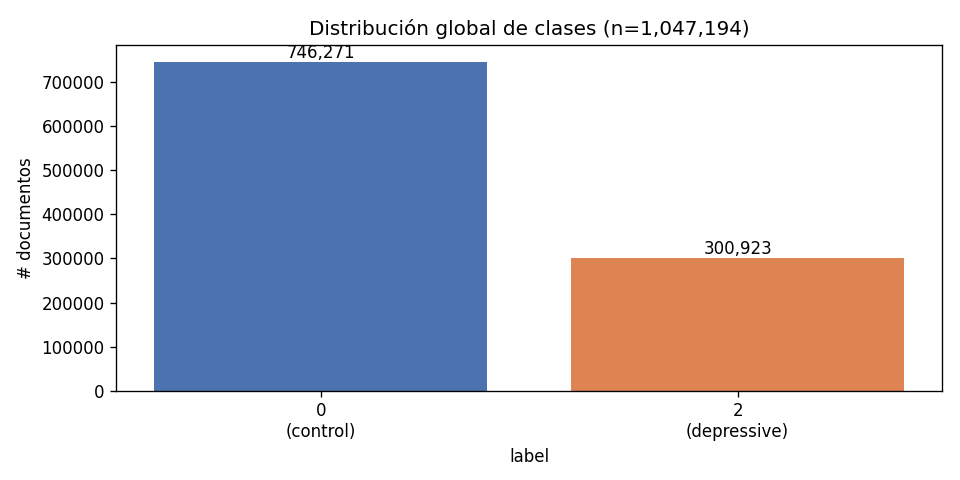
\includegraphics[width=\textwidth,height=0.34\textheight,keepaspectratio]{eda_02_distribucion_clases.png}
    \end{figure}
  \end{columns}
  \ugrblock{Delimitación clave}{
    Se evalúan \textbf{modelos de clasificación de texto}; el sistema no es una herramienta de diagnóstico.
  }
\end{frame}

\begin{frame}{Planteamiento del problema}
  \ugrsubtitle{Pregunta de investigación central}
  \begin{quote}
    \emph{¿Es posible desarrollar un clasificador supervisado en Ciencia de Datos que, a partir de texto en español a nivel de documento, distinga publicaciones de la clase positiva (indicios de depresión) frente a controles con un desempeño predictivo superior al de las representaciones clásicas, manteniendo robustez y evaluación no sesgada?}
  \end{quote}
  \ugrblock{Preguntas derivadas}{
    \begin{itemize}
      \item ¿Mitiga la traducción automática la escasez de datos en español?
      \item ¿Aprenden los clasificadores marcadores regionales espurios en lugar de señales del contenido?
    \end{itemize}
  }
\end{frame}

\begin{frame}{Hipótesis general y nula}
  \footnotesize
  \ugrsubtitle{Criterio de contraste formal}
  \begin{columns}[t]
    \column{0.49\textwidth}
    \ugrblockok{$H_1$ (general)}{
      Un modelo de lenguaje contextual en español \textbf{supera} el rendimiento predictivo de los modelos lineales léxicos.
    }
    \column{0.49\textwidth}
    \ugrblock{$H_0$ (nula)}{
      Un modelo de lenguaje contextual en español \textbf{no presenta diferencias significativas} en su rendimiento predictivo respecto de los modelos lineales léxicos.
    }
  \end{columns}
  \ugrblock{Criterio de decisión (bootstrap pareado, $B=2000$, $\alpha=0{,}05$)}{
    Rechazar $H_0$ a favor de $H_1$ si y solo si
    $\Delta F_{1,\text{low}} > 0 \;\land\; \Delta\text{AUC}_{\text{low}} > 0$.
    Intervalo de confianza del 95\,\% de la diferencia pareada BETO vs.\ mejor línea base léxica.
  }
\end{frame}

\begin{frame}{Objetivos}
  \ugrsubtitle{Objetivo general y específicos}
  \begin{multicols}{2}
    \begin{itemize}
      \item Consolidar y caracterizar un corpus textual a gran escala en español.
      \item Implementar clasificadores: TF-IDF + LR/SVM, rasgos lingüísticos y BETO.
      \item Evaluar con métricas multidimensionales sobre particiones a nivel de usuario.
      \item Comparar entrenamiento nativo (mono) vs.\ ampliado (multi).
      \item Auditar sesgo dialectal e interpretar los rasgos más influyentes.
    \end{itemize}
  \end{multicols}
\end{frame}

\begin{frame}{Restricciones y desvíos justificados del plan}
  \ugrsubtitle{Evaluación de la situación}
  \begin{itemize}
    \item \textbf{Tarea binaria} (control vs.\ indicios de depresión) en lugar de tres niveles de riesgo: el corpus nativo solo tiene etiquetas binarias validadas.
    \item \textbf{Corpus de acceso restringido} (MentalRiskES, Leis et al.): se usa Coello-Guilarte más tres colecciones de Reddit traducidas.
    \item \textbf{Partición única 70/10/20 por usuario} en lugar de 5-fold: cinco pliegues de BETO exigirían casi 30 horas de GPU.
    \item \textbf{SHAP/LIME sobre BETO diferido}: se reemplaza por una prueba de enmascarado léxico.
  \end{itemize}
\end{frame}

% =====================================================================
% FASE 2. COMPRENSIÓN DE LOS DATOS
% =====================================================================
\section{Comprensión de los datos}
\begin{frame}{Corpus unificado}
  \small
  \ugrsubtitle{1,311,023 documentos de 260,357 usuarios}
  \begin{table}
    \centering\small
    \setlength{\tabcolsep}{4pt}
    \begin{tabular}{lrrrr}
      \toprule
      \textbf{Fuente} & \textbf{Documentos} & \textbf{\%} & \textbf{Idioma orig.} & \textbf{Etiqueta} \\
      \midrule
      Coello-Guilarte (Twitter) & 1\,047\,194 & 79{,}88 & español & Usuario (0 / 2) \\
      Kaggle SDD (Reddit) & 232\,067 & 17{,}70 & inglés (trad.) & Comunidad \\
      Reddit Mental Health Posts & 24\,031 & 1{,}83 & inglés (trad.) & Comunidad \\
      Depression Reddit & 7\,731 & 0{,}59 & inglés (trad.) & Comunidad \\
      \midrule
      \textbf{Total} & \textbf{1\,311\,023} & \textbf{100} & -- & 260\,357 usuarios \\
      \bottomrule
    \end{tabular}
  \end{table}
  \ugrblock{Anonimización}{
    URLs, menciones, correos, teléfonos eliminados; identificadores hasheados (SHA-256 truncado).
  }
\end{frame}

% =====================================================================
% FASE 3. PREPARACIÓN DE LOS DATOS
% =====================================================================
\section{Preparación de los datos}
\begin{frame}{Pasos de preparación}
  \ugrsubtitle{Del texto crudo al conjunto de modelado}
  \begin{itemize}
    \item \textbf{Anonimización:} URLs, menciones, correos y teléfonos eliminados; identificadores con SHA-256.
    \item \textbf{Traducción:} 263\,829 publicaciones de Reddit con MarianMT (\texttt{opus-mt-en-es}).
    \item \textbf{Rasgos:} 19 por documento (primera persona, absolutistas, emoción, polaridad, temporales); se excluyó el número de mensajes por usuario para evitar fuga.
    \item \textbf{Balanceo (solo entrenamiento):} submuestreo 50/50 (424\,436 filas en mono) o ponderación de clases (700\,717 filas).
    \item \textbf{Partición por usuario} 70/10/20: validación y prueba conservan la distribución original.
  \end{itemize}
\end{frame}

\begin{frame}{Partición a nivel de usuario (sin fuga de información)}
  \ugrsubtitle{Estratificación 70/10/20 por autor, semilla 42}
  \tikzdiagram{
    \begin{tikzpicture}[font=\footnotesize, x=1cm, y=1cm]
        \node[anchor=west] at (0, 1.3) {%
            \tikz\fill[ugrAzul] (0,0) rectangle (0.3,0.3); Entrenamiento (70\,\%)\qquad
            \tikz\fill[ugrCeleste] (0,0) rectangle (0.3,0.3); Validación (10\,\%)\qquad
            \tikz\fill[ugrNaranja] (0,0) rectangle (0.3,0.3); Prueba (20\,\%)};
        \foreach \y/\nombre/\info in {
            0/Coello-Guilarte/317 usuarios,
            -1.05/Kaggle SDD/232\,067 usuarios sintéticos,
            -2.1/Reddit MH Posts/20\,242 usuarios,
            -3.15/Depression Reddit/7\,731 usuarios sintéticos} {
            \node[anchor=east, align=right] at (-0.25, \y) {\textbf{\nombre}\\[-1pt] {\color{ugrGris}\info}};
            \fill[ugrAzul]    (0, \y - 0.32) rectangle (7, \y + 0.32);
            \fill[ugrCeleste] (7, \y - 0.32) rectangle (8, \y + 0.32);
            \fill[ugrNaranja] (8, \y - 0.32) rectangle (10, \y + 0.32);
            \draw[white, line width=1.4pt] (7, \y - 0.32) -- (7, \y + 0.32) (8, \y - 0.32) -- (8, \y + 0.32);
            \node[text=white, font=\scriptsize\bfseries] at (3.5, \y) {usuarios completos, estratificados por clase};
        }
        \draw[ugrRojo, line width=1.1pt, dashed, rounded corners=2pt] (7.92, -0.42) rectangle (10.08, 0.42);
        \node[ugrRojo, anchor=south, font=\scriptsize\bfseries] at (9.0, 0.44) {test nativo común};
        \draw[decorate, decoration={brace, amplitude=5pt}, line width=0.8pt, ugrAzul] (10.35, 0.36) -- (10.35, -0.36)
            node[midway, right=7pt, text=ugrAzul] {\textbf{splits mono}};
        \draw[decorate, decoration={brace, amplitude=7pt}, line width=0.8pt, ugrNaranja!90!black] (12.75, 0.42) -- (12.75, -3.5)
            node[midway, right=9pt, align=left, text=ugrNaranja!90!black] {\textbf{splits multi}\\ unión de las\\ cuatro fuentes};
    \end{tikzpicture}
  }
  \ugrblock{Protocolo}{
    64 usuarios nunca vistos en el conjunto de prueba nativo (250\,847 textos).
  }
\end{frame}

% =====================================================================
% FASE 4. MODELADO
% =====================================================================
\section{Modelado}
\begin{frame}{Jerarquía de modelos supervisados}
  \ugrsubtitle{Tres niveles de complejidad representacional}
  \begin{columns}[t]
    \column{0.55\textwidth}
    \begin{itemize}
      \item \textbf{Líneas base léxicas:} TF-IDF (unigramas + bigramas, 15\,000 términos) con Regresión Logística y SVM lineal.
      \item \textbf{Modelo combinado:} TF-IDF + 19 rasgos lingüísticos/temporales + Regresión Logística.
      \item \textbf{Modelo contextual:} BETO (\texttt{dccuchile/bert-base-spanish-wwm-cased}), 110M parámetros, ajuste fino en GPU local RTX 3060 Ti (8\,GB).
    \end{itemize}
    \column{0.42\textwidth}
    \tikzdiagram{
      \begin{tikzpicture}[font=\footnotesize, node distance=0.55cm]
          \node[proceso=2.6cm, fill=ugrGris!8, draw=ugrGris] (tx) {\textbf{Texto}\\ \emph{``no me}\\ \emph{siento bien''}};
          \node[proceso=2.6cm, right=of tx] (tok) {\textbf{Tokenización}\\ WordPiece\\ \texttt{[CLS]} \dots{} \texttt{[SEP]}\\ máx.\ 128 tokens};
          \node[proceso=2.9cm, right=of tok, minimum height=2.6cm, fill=ugrAzul!10, line width=0.9pt] (enc)
              {\textbf{BETO}\\ codificador Transformer\\ 12 capas $\times$ 12 cabezas\\ $d = 768$\\ {\color{ugrGris}\scriptsize preentrenado, se ajusta}};
          \node[proceso=2.2cm, right=of enc] (cls) {\textbf{Vector}\\ $h_{\texttt{[CLS]}} \in \mathbb{R}^{768}$};
          \node[proceso=2.2cm, right=of cls, draw=ugrNaranja, fill=ugrNaranja!8] (lin) {\textbf{Capa lineal}\\ $768 \to 2$\\ + softmax};
          \node[resultado=2.9cm, below=0.7cm of lin] (out) {$P(y=1\mid x)$};
          \draw[flecha] (tx) -- (tok);
          \draw[flecha] (tok) -- (enc);
          \draw[flecha] (enc) -- (cls);
          \draw[flecha] (cls) -- (lin);
          \draw[flecha] (lin) -- (out);
          \node[below=0.15cm of enc, font=\scriptsize, text=ugrGris, align=center] {AdamW, $\eta = 2\times10^{-5}$, lote 16, FP16};
      \end{tikzpicture}
    }
    {\scriptsize\centering Arquitectura del ajuste fino de BETO.\par}
  \end{columns}
\end{frame}

\begin{frame}{Transformers: atención y Regresión Logística}
  \ugrsubtitle{Representaciones contextuales vs. léxicas}
  \begin{columns}[t]
    \column{0.52\textwidth}
    \begin{equation}
      \operatorname{Attention}(Q,K,V) =
      \operatorname{softmax}\!\left(\frac{QK^{\top}}{\sqrt{d_k}}\right)V
    \end{equation}
    BETO: 12 capas, 12 cabezas, $d=768$, Whole Word Masking.
    \column{0.45\textwidth}
    \begin{equation}
      P(y=1\mid x) = \sigma(w^{\top}x + b)
    \end{equation}
    Regresión Logística con $L_2$; coeficientes inspeccionables por término.
  \end{columns}
\end{frame}

% =====================================================================
% FASE 5. EVALUACIÓN
% =====================================================================
\section{Evaluación}
\begin{frame}{Protocolo de evaluación y métricas}
  \ugrsubtitle{F1-macro y AUC-ROC con bootstrap de usuarios}
  \begin{columns}[t]
    \column{0.55\textwidth}
    \begin{itemize}
      \item Métrica principal: \textbf{F1-macro} (equilibrado ante desbalance de clases).
      \item Métrica robusta: \textbf{AUC-ROC} (independiente del umbral).
      \item Métrica de acuerdo: $\kappa$ de Cohen.
    \end{itemize}
    \column{0.42\textwidth}
    \begin{equation}
      \text{F1-macro} = \tfrac{1}{2}\left(\text{F1}_{\text{control}} + \text{F1}_{\text{depresión}}\right)
    \end{equation}
  \end{columns}
  \ugrblock{Incertidumbre: bootstrap por conglomerados de usuarios}{
    2\,000 réplicas remuestreando usuarios (no textos). Intervalos percentiles del 95\,\%. Unidad efectiva: el usuario (64 en prueba nativa).
  }
\end{frame}

% =====================================================================
% 5. RESULTADOS PRINCIPALES
% =====================================================================
\begin{frame}{Resultados sobre el test nativo común}
  \ugrsubtitle{BETO mono vs. líneas base léxicas (250\,847 textos, 64 usuarios)}
  \begin{table}
    \centering\footnotesize
    \setlength{\tabcolsep}{3.5pt}
    \caption{Métricas con IC 95\,\% (bootstrap de 64 usuarios).}
    \begin{tabular}{lrrrr}
      \toprule
      \textbf{Modelo} & \textbf{F1-macro} & \textbf{F1 dep.} & \textbf{AUC} & $\boldsymbol{\kappa}$ \\
      \midrule
      LR TF-IDF (ponderación) & 0{,}655 {[0{,}606; 0{,}693]} & 0{,}546 & 0{,}755 {[0{,}718; 0{,}790]} & 0{,}321 \\
      SVM TF-IDF & 0{,}653 {[0{,}605; 0{,}692]} & 0{,}544 & 0{,}754 {[0{,}716; 0{,}787]} & 0{,}318 \\
      \cellcolor{filaResaltada}\textbf{BETO mono} & \cellcolor{filaResaltada}\textbf{0{,}717} {[0{,}665; 0{,}759]} & \cellcolor{filaResaltada}\textbf{0{,}613} & \cellcolor{filaResaltada}\textbf{0{,}808} {[0{,}755; 0{,}849]} & \cellcolor{filaResaltada}\textbf{0{,}437} \\
      \bottomrule
    \end{tabular}
  \end{table}
  \ugrblockok{Mejoría de BETO sobre la mejor línea base}{
    $\Delta$F1-macro = +0{,}062 {[0{,}038; 0{,}081]} $\cdot$ $\Delta$AUC = +0{,}052 {[0{,}024; 0{,}077]}. Ambos intervalos excluyen estrictamente el cero.
  }
\end{frame}

\begin{frame}{Curvas ROC y matriz de confusión (BETO mono)}
  \ugrsubtitle{Capacidad de discriminación y errores}
  \begin{columns}[t]
    \column{0.50\textwidth}
    \begin{figure}
      \centering
      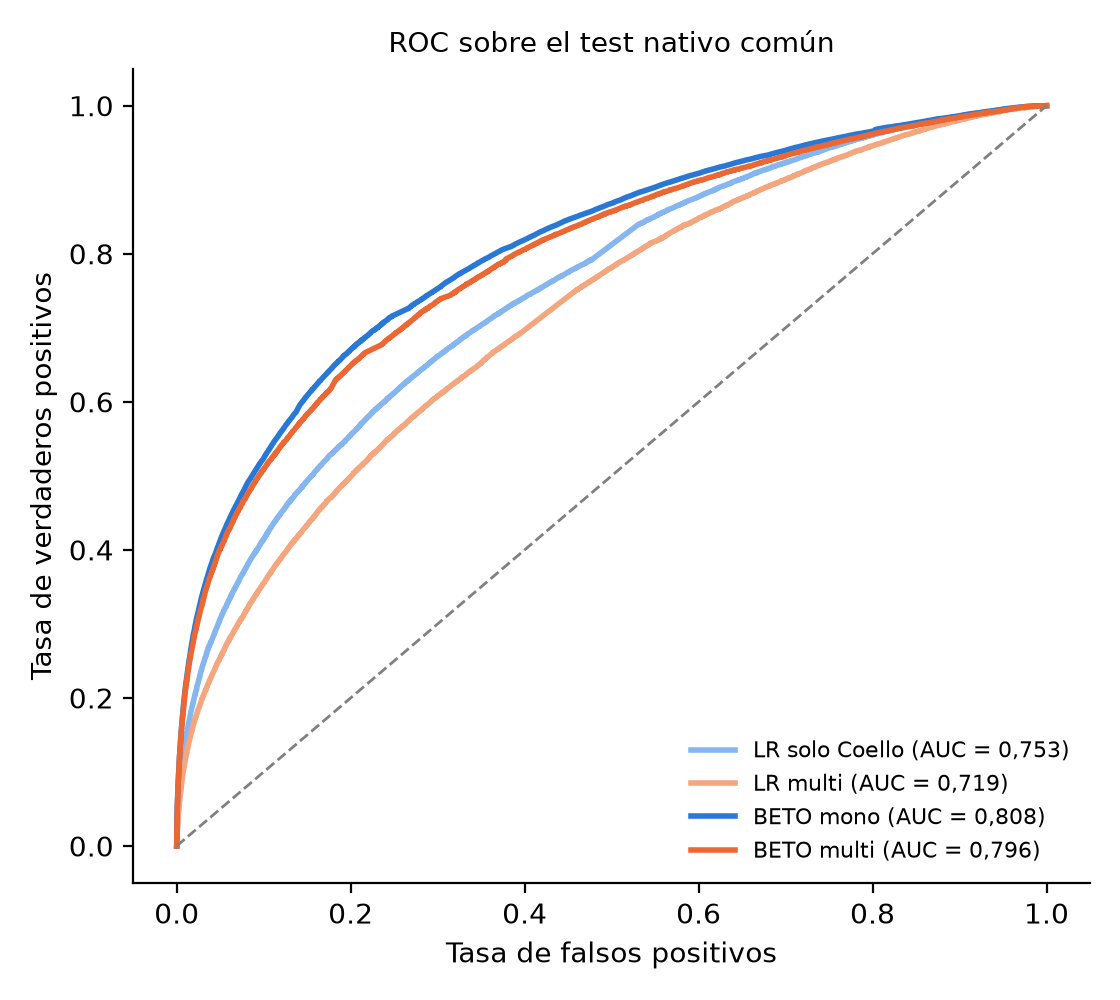
\includegraphics[width=\textwidth,height=0.54\textheight,keepaspectratio]{roc_test_nativo.png}
      \caption{Curvas ROC, test nativo.}
    \end{figure}
    \column{0.50\textwidth}
    \begin{figure}
      \centering
      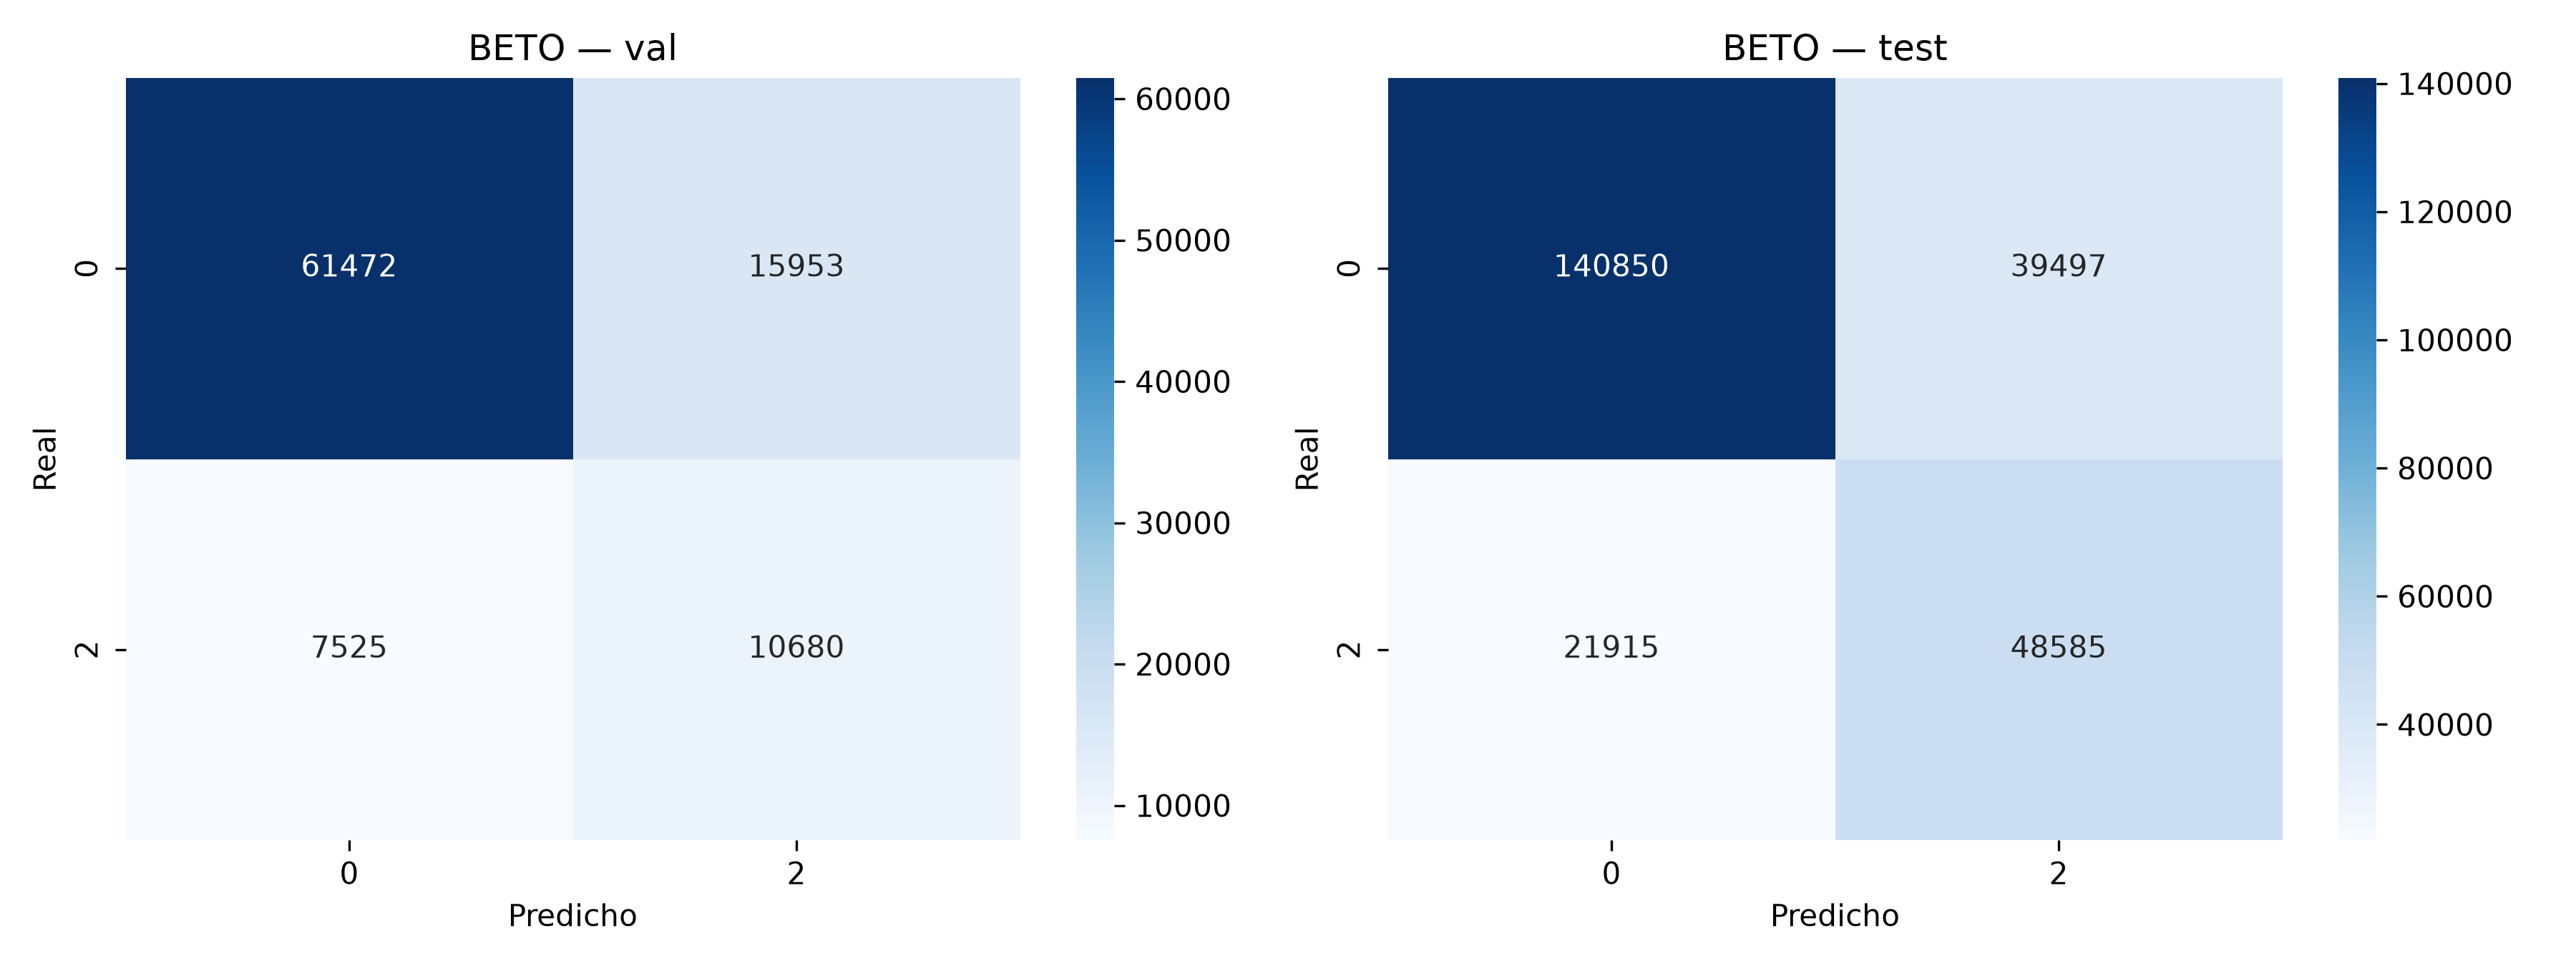
\includegraphics[width=\textwidth,height=0.54\textheight,keepaspectratio]{beto_confusion_matrix.png}
      \caption{Matriz de confusión, prueba.}
    \end{figure}
  \end{columns}
\end{frame}

\begin{frame}{Contrastación formal de la hipótesis ($H_1$ vs.\ $H_0$)}
  \ugrsubtitle{Diferencias pareadas por bootstrap de usuarios}
  \begin{table}
    \centering\footnotesize
    \setlength{\tabcolsep}{4pt}
    \caption{Diferencias pareadas (A $-$ B), IC 95\,\% bootstrap de usuarios.}
    \begin{tabular}{lrrr}
      \toprule
      \textbf{Comparación} & $\Delta$ F1-macro & $\Delta$ AUC & $\Delta\,\kappa$ \\
      \midrule
      BETO mono $-$ LR mono & +0{,}062 {[0{,}038; 0{,}081]} & +0{,}052 {[0{,}024; 0{,}077]} & +0{,}116 {[0{,}068; 0{,}155]} \\
      BETO mono $-$ SVM mono & +0{,}063 {[0{,}040; 0{,}081]} & +0{,}054 {[0{,}026; 0{,}077]} & +0{,}119 {[0{,}072; 0{,}156]} \\
      \bottomrule
    \end{tabular}
  \end{table}
  \ugrblockok{Decisión formal}{
    \textbf{Se rechaza $H_0$ y se acepta $H_1$} a nivel de publicación: BETO supera consistentemente a las líneas base léxicas en todas las métricas y en el 100\,\% de las réplicas de bootstrap.
  }
\end{frame}

% =====================================================================
% 6. TRADUCCIÓN Y DOMINIOS
% =====================================================================
\begin{frame}{Efecto del aumento de datos mediante traducción (mono vs.\ multi)}
  \ugrsubtitle{¿Mejora traducir datos de inglés al español?}
  \begin{table}
    \centering\footnotesize
    \setlength{\tabcolsep}{3pt}
    \caption{F1-macro y AUC por fuente del test multi.}
    \begin{tabular}{lrrrr}
      \toprule
      \textbf{Modelo} & \multicolumn{2}{c}{\textbf{Nativo}} & \multicolumn{2}{c}{\textbf{Kaggle SDD (Reddit)}} \\
      & F1-M & AUC & F1-M & AUC \\
      \midrule
      BETO mono & \textbf{0{,}717} & \textbf{0{,}808} & 0{,}415 & 0{,}801 \\
      BETO multi & 0{,}701 & 0{,}796 & \textbf{0{,}934} & \textbf{0{,}986} \\
      \bottomrule
    \end{tabular}
  \end{table}
  \ugrblock{Hallazgo principal}{
    Sobre texto nativo, agregar datos traducidos \emph{no mejora} (BETO: 0{,}717 $\rightarrow$ 0{,}701). Sobre el dominio traducido, los datos traducidos son \emph{imprescindibles} (F1: 0{,}415 $\rightarrow$ 0{,}934).
  }
\end{frame}

\begin{frame}{Diseño experimental: dos dominios de prueba}
  \ugrsubtitle{Mismo modelo, dos fuentes de prueba}
  \tikzdiagram{
    \begin{tikzpicture}[font=\footnotesize]
        \node[font=\footnotesize\bfseries, text=ugrAzul] at (-0.6, 1.25) {Datos de entrenamiento};
        \node[font=\footnotesize\bfseries, text=ugrAzul] at (3.0, 1.25) {TF-IDF + LR};
        \node[font=\footnotesize\bfseries, text=ugrAzul] at (6.0, 1.25) {BETO};
        \node[nodoES, text width=3.3cm] (dmono) at (-0.6, 0.35) {\textbf{Mono}\\ solo tweets nativos};
        \node[nodoEN, text width=3.3cm] (dmulti) at (-0.6, -1.15) {\textbf{Multi}\\ tweets nativos +\\ Reddit traducido};
        \node[proceso=2.4cm] (lrm)  at (3.0,  0.35) {LR mono};
        \node[proceso=2.4cm] (btm)  at (6.0,  0.35) {BETO mono};
        \node[proceso=2.4cm] (lrx)  at (3.0, -1.15) {LR multi};
        \node[proceso=2.4cm] (btx)  at (6.0, -1.15) {BETO multi};
        \draw[flecha] (dmono) -- (lrm);
        \draw[flecha] (dmulti) -- (lrx);
        \begin{scope}[on background layer]
            \node[draw=ugrAzul!45, dashed, rounded corners=4pt, fill=ugrAzul!3, inner sep=7pt, fit=(lrm)(btm)(lrx)(btx)] (grp) {};
        \end{scope}
        \node[resultado=4.4cm] (tn) at (11.4, 0.35) {\textbf{Test nativo común}\\ 250\,847 tweets $\cdot$ 64 usuarios};
        \node[resultado=4.4cm, draw=ugrNaranja, fill=ugrNaranja!8] (tt) at (11.4, -1.15) {\textbf{Test traducido}\\ 52\,757 textos de Reddit};
        \draw[flecha] (grp.east |- tn) -- (tn) node[midway, above, font=\scriptsize, text=ugrGris] {todos};
        \draw[flecha] (grp.east |- tt) -- (tt) node[midway, below, font=\scriptsize, text=ugrGris] {todos};
    \end{tikzpicture}
  }
  \ugrblock{Implicación}{
    Una métrica agregada sobre un conjunto multifuente oculta que el modelo es excelente en el dominio traducido pero ligeramente peor en el nativo.
  }
\end{frame}

% =====================================================================
% 7. AUDITORÍA DE SESGO
% =====================================================================
\begin{frame}{Control experimental: enmascarado de marcadores diatópicos}
  \small
  \ugrsubtitle{¿Dependen los modelos de marcadores regionales en lugar de señales del contenido?}
  \begin{table}
    \centering\scriptsize
    \setlength{\tabcolsep}{4pt}
    \begin{tabular}{lrrr}
      \toprule
      \textbf{Modelo} & \textbf{Condición} & $\Delta$ F1-macro & $\Delta$ AUC \\
      \midrule
      LR mono & Original & -- & -- \\
      & Todos los marcadores & $-0{,}015$ & $-0{,}025$ \\
      & Control aleatorio & $\approx 0$ & $\approx 0$ \\
      \midrule
      BETO mono & Original & -- & -- \\
      & Todos los marcadores & $-0{,}014$ & $-0{,}021$ \\
      & Control aleatorio & $\approx 0$ & $\approx 0$ \\
      \bottomrule
    \end{tabular}
  \end{table}
  \ugrblock{Conclusiones}{
    \begin{itemize}
      \item Todos los modelos, BETO incluido, dependen de marcadores dialectales/geográficos.
      \item Enmascararlos reduce el AUC 2 a 2{,}5 puntos; el control aleatorio no tiene efecto.
      \item El sesgo regional \emph{no explica} la ventaja relativa de BETO.
    \end{itemize}
  }
\end{frame}

% =====================================================================
% 8. NIVEL DE USUARIO E INTERPRETABILIDAD
% =====================================================================
\begin{frame}{Agregación a nivel de usuario (64 usuarios, 19 positivos)}
  \ugrsubtitle{Del tweet al perfil de usuario}
  \begin{table}
    \centering\footnotesize
    \setlength{\tabcolsep}{4pt}
    \caption{Métricas agregando el puntaje medio de cada usuario.}
    \begin{tabular}{lrrr}
      \toprule
      \textbf{Modelo} & \textbf{F1-macro} & \textbf{AUC} & $\boldsymbol{\kappa}$ \\
      \midrule
      LR mono & 0{,}925 & 0{,}989 & 0{,}850 \\
      SVM mono & 0{,}943 & 0{,}989 & 0{,}886 \\
      BETO mono & 0{,}888 & 0{,}982 & 0{,}775 \\
      \bottomrule
    \end{tabular}
  \end{table}
  \ugrblock{Observación}{
    El AUC sube de 0{,}72--0{,}81 (por publicación) a 0{,}98--0{,}99 (por usuario), pero la ventaja de BETO \emph{desaparece}.
  }
\end{frame}

\begin{frame}{¿Qué aprende el modelo léxico? Interpretabilidad}
  \small
  \ugrsubtitle{Términos más predictivos de la Regresión Logística}
  \begin{columns}[t]
    \column{0.54\textwidth}
    \begin{itemize}
      \item Términos más predictivos son \textbf{marcadores dialectales y geográficos}, no del contenido:
        \emph{wey, mexicanos, puebla} (control, México) vs.\ \emph{vos, joder, uribe, colombia} (clase positiva).
      \item Ninguno de los 30 términos extremos es un rasgo lingüístico de la literatura.
    \end{itemize}
    \column{0.43\textwidth}
    \begin{figure}
      \centering
      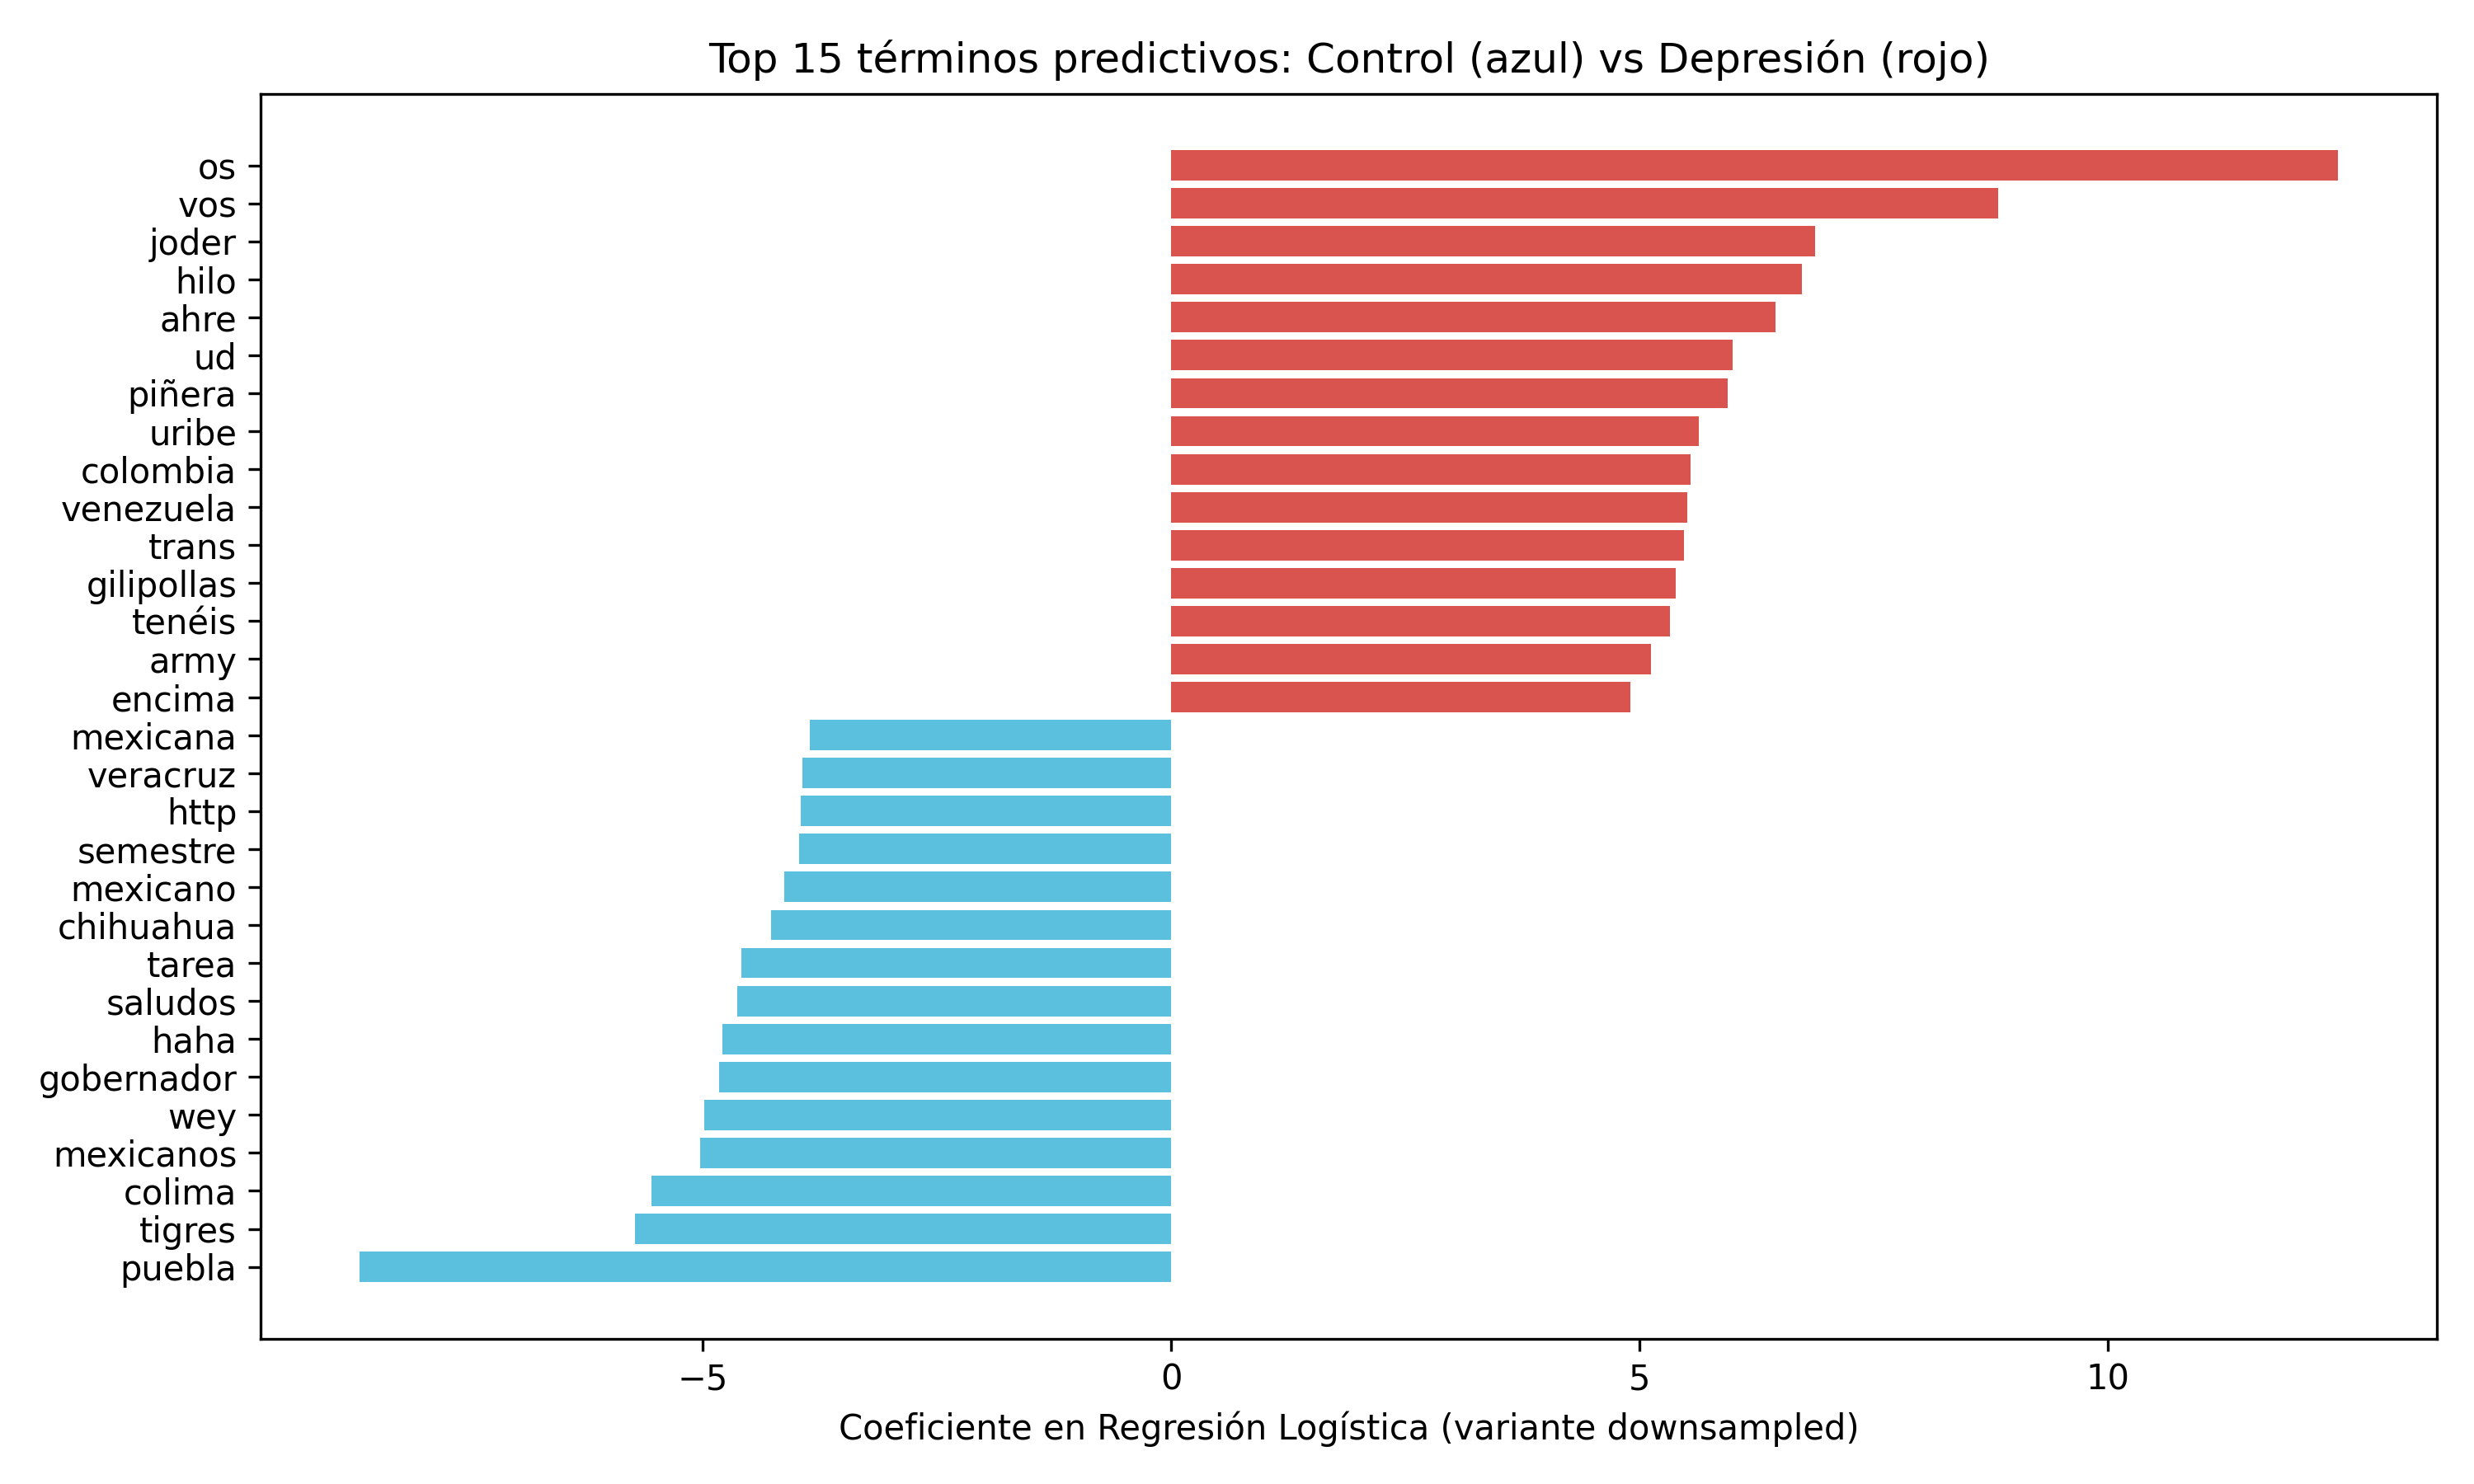
\includegraphics[width=\textwidth,height=0.34\textheight,keepaspectratio]{baseline_downsampled_top_features.png}
    \end{figure}
  \end{columns}
  \ugrblock{Rasgos léxicos (diferencia relativa en la clase positiva)}{
    Emoción negativa: $+62$\,\% ($p=0{,}003$); emoción positiva: $-32$\,\%. Primera persona: $-3$\,\%; absolutistas: $+2$\,\%.
  }
\end{frame}



\section{Despliegue y cierre}
\begin{frame}{Despliegue: replicabilidad y uso responsable}
  \ugrsubtitle{Transferencia sin puesta en producción clínica}
  \begin{itemize}
    \item Código, manifiestos de partición y predicciones públicos: las métricas se recalculan sin reentrenar.
    \item Semillas fijas (42), dependencias declaradas y un objetivo de \texttt{make} por etapa.
    \item Datos públicos y anonimizados antes de cualquier análisis; sin intento de reidentificación.
    \item Transparencia sobre limitaciones y sesgos detectados.
    \item Los modelos son clasificadores estadísticos: \textbf{no constituyen diagnóstico}.
    \item Cualquier uso aplicado requeriría validación externa con anotación experta.
  \end{itemize}
\end{frame}

% =====================================================================
% CONCLUSIONES
% =====================================================================
\begin{frame}{Conclusiones}
  \ugrsubtitle{Resumen de hallazgos}
  {\small
    \begin{itemize}
      \item \textbf{BETO supera a líneas base léxicas} a nivel de publicación: F1-macro 0{,}717 vs.\ 0{,}655; AUC 0{,}808 vs.\ 0{,}755. \textbf{$H_0$ rechazada, $H_1$ aceptada}.
      \item La traducción automática \emph{no mejora} el dominio nativo, pero es \emph{imprescindible} para el dominio traducido (Reddit: 0{,}934 vs.\ 0{,}415).
      \item La partición por usuario y la evaluación desagregada por fuente son requisitos de validez.
      \item Todos los modelos dependen de marcadores dialectales (caída de 2--2{,}5 puntos de AUC).
      \item La agregación por usuario lleva el AUC a $\geq 0{,}98$, diluyendo la ventaja de BETO.
    \end{itemize}}
  \ugrblockok{Alcance}{
    Comparación empírica de modelos de clasificación de texto. \emph{No} es una herramienta de diagnóstico individual.
  }
\end{frame}

\begin{frame}{Trabajo futuro}
  \ugrsubtitle{Líneas de extensión}
  \begin{itemize}
    \item Control del sesgo geográfico: reentrenar con marcadores dialectales enmascarados; corpus balanceado por país.
    \item Aumento orientado al dominio nativo: preentrenamiento en traducido + ajuste fino solo en tweets.
    \item Detección temprana secuencial a nivel de usuario (protocolo eRisk).
    \item Explicabilidad de BETO: SHAP, LIME y análisis de atención.
    \item Corpus con anotación experta y otros modelos (XLM-RoBERTa, MarIA, RoBERTa-BNE).
  \end{itemize}
\end{frame}

% =====================================================================
% CIERRE
% =====================================================================
\begin{frame}[plain]
  \begin{tikzpicture}[remember picture,overlay]
    \fill[ugrAzul] (current page.north west) rectangle (current page.south east);
    \node[anchor=center] at (current page.center) {
      \begin{minipage}{0.8\textwidth}
        \centering
        \color{white}\Huge\bfseries Gracias por su atención\par\medskip
        \color{ugrCeleste!10}\large Preguntas y comentarios\par\medskip
        \color{white}\rule{0.6\textwidth}{1pt}\par\medskip
        \color{ugrCeleste!30}\small Código y datos: \texttt{https://github.com/giulicrenna/Deteccion-Temprana-Depresion}\par\medskip
        \color{ugrCeleste!30}\small Giuliano Crenna · Bruno Emmanuel Pace — UGR, 2026
      \end{minipage}};
  \end{tikzpicture}
\end{frame}

\end{document}

